
\chapter{Interpreting Data}

Let's take an intermission from the nitty-gritty Python stuff and talk about
how to properly \textit{interpret} the data we're working with; specifically,
how to draw correct conclusions from what we've collected.

\section{Independent and dependent variables}

\index{variable!dependent}
\index{variable!independent}
\index{independent variable (i.v.)}
\index{dependent variable (d.v.)}
\index{cause}
\index{causal}
\index{hiccup}
\index{greenhouse gas}
\index{smoking}
\index{lung cancer}
\index{global warming}

You've undoubtedly seen countless studies that claim to reveal important truths
about the world, such as that smoking can cause lung cancer, greenhouse gas
emissions can cause higher global temperatures, or orgasms can cure hiccups.
Much of the time, scientists try to find a \textbf{causal} factor that links
one variable to another: they suspect that the value of a variable $A$ (often
called the \textbf{independent variable}, or ``\textbf{i.v.}''~for short) is a
\textit{reason}, or \textbf{cause}, of a certain value in another variable $B$
(the \textbf{dependent variable}, or ``\textbf{d.v.}'').

Just to avoid misunderstandings, when we claim that $A$ \textbf{causes} $B$, we
don't normally mean that it \textit{exclusively} causes it, or even that it
\textit{reliably} causes it. There are lots of contributing factors to lung
cancer besides smoking, after all; and tons of smokers never develop cancer. We
simply mean that $A$ is a contributing factor to $B$, and that the value of the
$A$ variable exerts some, but not total, influence over the value of the $B$
variable.

\index{variable}
\index{objects (of a study)}

Importantly, we're using the word \textbf{variable} here in a different, but
related way than we used it in chapters~\ref{ch:atomicData},
\ref{ch:arraysInPython1}, and \ref{ch:arraysInPython2}. As we did in
chapter~\ref{ch:scalesOfMeasure} (see p.~\pageref{variableDifferent} footnote),
we use ``variable'' here to mean a specific aspect of the \textbf{objects of a
study} that can differ, or ``vary.'' The objects in our study (often people,
but sometimes companies, organizations, environments, nations, \textit{etc.})
\textit{each} have a value for the variable. Thus if you think of a
``per-capita income'' variable, you might think of an entire \textit{array} of
floats, each of which represented the average income-per-resident of a single
nation.

\index{scales of measure}
\index{categorical variable}

The variables in question can be from any of the scales of measure from
chapter~\ref{ch:scalesOfMeasure}. Take the smoking example, with patients as
the object of study. We might say that independent variable $A$ is categorical,
with values \texttt{SMOKER} and \texttt{NON-SMOKER}. The dependent variable $B$
is also categorical: \texttt{CANCER} and \texttt{NO-CANCER}. The key question
is: do people with $A=\texttt{SMOKER}$ also have $B=\texttt{CANCER}$
\textit{more often} (a higher percentage of the time) than people with
$A=\texttt{NON-SMOKER}$ do?

\index{ratio variable}
\index{interval variable}

In the greenhouse gas emissions example, our objects of study might be
\textit{years}. Our variables are both numeric, with $A$ (a measure of yearly
greenhouse gas emissions, measured in gigatonnes $\textrm{CO}_2$) on the ratio
scale, and $B$ (average worldwide temperature increase/decrease) on an interval
scale. Here, the question would be: do years in which $A$ is relatively high
typically also have $B$ relatively high? Put another way: do years in which
earthlings have released more gas into the atmosphere tend to correspond with
years in which the global temperature increased?

And of course, we might have one categorical variable and one numeric. Perhaps
our objects of study are American adults, and while our categorical $A$
variable has values \texttt{DEMOCRAT}, \texttt{REPUBLICAN}, \texttt{OTHER}, and
\texttt{INDEPENDENT}, our numerical $B$ is yearly income. Our question would
be: do adherents of one political party tend to be more wealthy than those of
another?

Or, flipping sides, the independent variable $A$ could be numeric while the
dependent variable $B$ is categorical. Our objects of study might be high
school seniors applying to UMW. Let $A$ be the number of different colleges a
student applied to, and $B$ a categorical variable with values
\texttt{ADMITTED-TO-UMW} and \texttt{NOT-ADMITTED-TO-UMW}. The question of
interest is here is: do students who apply to more colleges tend to get in to
UMW more often?

\section{Association and causality}

\label{association}

All of the above questions can be answered with data. In future chapters, we'll
learn the exact Python commands to ask them, and how to interpret the answers.

\index{association}
\index{correlation}
\index{dependent}

For now, I merely want to draw your attention to the fact that these are all
questions of \textbf{association}, not causation. An association between
variables merely means that they are \textbf{correlated} in some way
statistically.\footnote{Another way to put this is to say that the variables
are \textbf{dependent} on each other, although this is confusing because we're
already using the word ``dependent'' to refer to one of the variables.} If
$A=\texttt{SMOKER}$ goes with $B=\texttt{CANCER}$ more often than
$A=\texttt{NON-SMOKER}$ does, then there \textit{is} an association between the
two, period. If yearly income $B$ is on average higher for
$A=\texttt{REPUBLICAN}$ than for $A=\texttt{DEMOCRAT}$, then there \textit{is}
an association between the two, period.

\label{howMuchMore}

(By the way, a key nuance will turn out to be: \textit{how much} more often
does $A=\texttt{SMOKER}$ need to go with $B=\texttt{CANCER}$ in order for us to
be confident that there is a true association? Or \textit{how much} more
wealthy do the $A=\texttt{REPUBLICAN}$s need to be on average for us to have
confidence we've identified a real link to political party? That one's a little
tricky, and we'll postpone addressing it for now.)

\index{causality}
\label{pythonAssociation}

So anyway, the question of association turns out to be pretty straightforward
to answer. Python will simply tell us if variables are associated or not. More
difficult, however, is determining \textbf{causality}
(a.k.a.~\textbf{causation}). Does a person's political affiliation influence
how much wealth they have? Or is it the other way around: does a person's
wealth cause them to vote a certain way? Or is it neither of these, with some
third factor (perhaps values, or life philosophy) helping determine
\textit{both} variables?

\index{$\rightarrow$@$\rightarrow$ (causality)}

If the first of these three is the case, we would write ``$A \rightarrow B$,''
pronounced ``$A$ causes $B$''. If the second, we'd write, ``$B \rightarrow
A$,'' and for the third, we'd write ``$C \rightarrow A, B$'' for some other
(possibly yet to be determined) variable $C$. Determining which (if any) of
these is true calls for some careful thinking, intuition, and additional kinds
of statistical tests.

In fact, just to blow your mind, Figure~\ref{fig:causalityTypes} gives a
partial list of the various types of causation that \textit{could} be the true
explanation, once we find out that $A$ and $B$ have an association. As you can
see, there are a lot of ways to go wrong. Only \textit{one} of the
possibilities is that ``$A$ actually causes $B$,'' which is what we suspected
in the first place. The others are all ways of producing that same association
we picked up in the data.

\begin{figure}[ht]
\footnotesize
\centering
\begin{tabular}{|c|c|p{2in}|}
\hline
Symbology & Name & Example \\
\hline
\multirow[c]{2}{*}{$A \rightarrow B$} & \multirow[c]{2}{*}{causation} & Regular
exercise does indeed normally lead to a lower resting heart rate. \\
\hline
\multirow[c]{2}{*}{$B \rightarrow A$} & \multirow[c]{2}{*}{reverse causation} & Smoking doesn't cause depression;
depression causes smoking. \\
\hline
\multirow[c]{2}{*}{$C \rightarrow A, B$} & \multirow[c]{2}{*}{\makecell{external causation \\ (confounding
factor)}} & Ice cream sales don't cause shark attacks; high temperatures boost both ice
cream sales and ocean swimming. \\
\hline
\multirow[c]{2}{*}{$A \rightarrow B$ \& $C \rightarrow B$} &
\multirow[c]{2}{*}{multiple causation }& A liberal arts
education does improve critical thinking skills, but lots of other things do
too. \\
\hline
\multirow[c]{2.5}{*}{$A,C \rightarrow B$} & \multirow[c]{2.5}{*}{joint causation} &
Just being tall doesn't necessarily make you a good basketball player, but if
your height is accompanied by another factor as well (athleticism), then you
will be. \\
\hline
\multirow[c]{2.5}{*}{$A \rightarrow C \rightarrow B$} &
\multirow[c]{2.5}{*}{indirect causation} & People who use antiperspirant tend to
get more dates, but it's not because of the antiperspirant \textit{per se};
it's because they don't have an unpleasant odor. \\
\hline
\multirow[c]{3}{*}{$A \not\rightarrow B$} & \multirow[c]{3}{*}{spurious
association} & Although for many years the outcome of the Washington football
game immediately preceding a Presidential election predicted the election's
outcome, that was by coincidence. \\
\hline
\end{tabular}
\medskip
\caption{Various types of causality that could be the underlying reason why an
association between $A$ and $B$ exists.}
\label{fig:causalityTypes}
\normalsize
\end{figure}
\vspace{-.15in}

\section{Confounding factors}

\index{confounding factor}
\index{external causation}
\index{variable!confounding}

Let me speak to two of the items in the Figure~\ref{fig:causalityTypes} table
in particular. The third one on the list, \textbf{external causation}, is a
case where a third variable (call it $C$) comes into play. We refer to this as
a \textbf{confounding factor} (or \textbf{confounding variable}) because it
``confounds'' us: causes us to interpret the meaning behind the data in an
incorrect way. The example in the table is a famous and funny one: clearly
sharks don't react to Ben \& Jerry's daily net profits, and people (probably)
don't run out and buy ice cream to cope with their anxiety about shark attacks.
Neither $A \rightarrow B$ nor $B \rightarrow A$, but a third variable -- hot
days -- influence both of them.

\begin{figure}[ht]
\centering
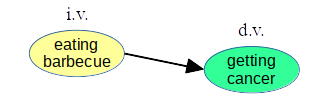
\includegraphics[width=0.6\textwidth]{causalDiagram.png}
\caption{A hypothesis as to causality: eating barbecued foods increases one's
risk for certain types of cancer.}
\label{fig:causalDiagram}
\end{figure}

\index{causal diagram}
\index{barbecue}
\index{cancer}
\label{barbecue}

% WARNING: "flip to"

Now of course it's not always this obvious. Here's an example I ran across
recently. A magazine article reported on a new health scare: scientists have
discovered that \textit{eating barbecue can increase your risk of cancer.}
Pictorially, this claim is illustrated in the \textbf{causal diagram} in
Figure~\ref{fig:causalDiagram} (flip to p.~\pageref{fig:causalDiagram}), which
shows our i.v.~and our d.v.~; the arrow means exactly what it meant earlier.

Unlike sharks and ice cream, this one seems plausible. And I'm not claiming to
have read enough about their study to tell whether the researchers' claim is
bogus. But I couldn't help thinking that there are a great many possibly
confounding factors that could be blurring the results. For one, choosing to
eat barbecue a lot is probably often associated with a less healthy, higher-fat
diet in general (I can speak from experience on that). If that's true, and if
high-fat diets -- whether featuring lots of barbecue or not -- are associated
with these same poor health outcomes, then we'd have the picture on the
left-side of Figure~\ref{fig:causalDiagram23} (also on
p.~\pageref{fig:causalDiagram23}). The red bubble represents the confounding
factor, which is influencing both i.v.~and d.v. If this picture were the
correct one of the underlying phenomenon, then the correlation we thought were
picking up between barbecue and cancer was actually due to fat content.

\begin{figure}[hb]
\centering
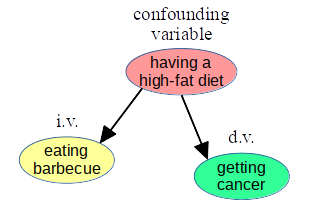
\includegraphics[width=0.4\textwidth]{causalDiagram2.png}
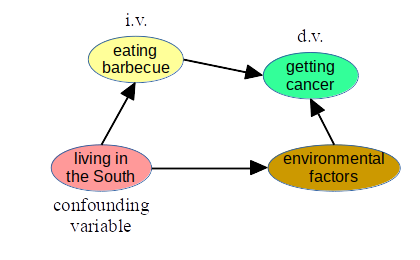
\includegraphics[width=0.5\textwidth]{causalDiagram3.png}
\caption{Other hypotheses as to causality, each resulting in the same
associations in the data, yet involving confounding factors.}
\label{fig:causalDiagram23}
\end{figure}

% WARNING: "below"

Another example is the right-hand side of Figure~\ref{fig:causalDiagram23},
below. Perhaps barbecue is more popular culturally in some areas of the country
(say, the South, where I certainly see it eaten a lot), and perhaps those areas
have other environmental factors that can lead to cancer. In this case, the
``South'' confounder indirectly affects the d.v.~(via another variable, the
environment) but it still affects it.

It's not hard to think of others. These were just the first two that came to
mind. The point is that it's really hard to be sure you've thought of all of
them!


\subsection{Paranoia and overparanoia}

All this should lead you to be somewhat paranoid, but not
\textit{over}\-paranoid. Confounding variables can definitely lead us to make
mistakes in our reasoning, but perhaps they're not \textit{quite} as common as
you think. Understand that a confounding factor is \textit{not} simply any
other factor that affects the dependent variable. Instead, for a variable to be
confounding \textbf{it must affect both the independent \textit{and} the
dependent variable.}

Let me illustrate with an example. I suspect that on average, men are taller
than women. And I further suspect that there's causality here, and that it goes
from $A$ (sex) to $B$ (height), not the other way around. (Clearly people don't
spontaneously ``turn male'' because they reach a certain height.) So my
thinking on the subject is summed up in Figure~\ref{fig:sexHeight}.

\vspace{-.15in}
\begin{figure}[ht]
\centering
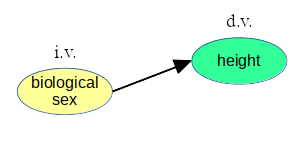
\includegraphics[width=0.6\textwidth]{sexHeight.png}
\caption{Stephen's hypothesis: a person's biological sex (male or female) plays
a causal role in determining their height.}
\label{fig:sexHeight}
\end{figure}

\smallskip
Now let me show you what I mean by ``overparanoia.'' What if someone said,
``but wait, Stephen, not so fast! You've got potential confounding variables
out the wazoo! Why, surely heredity plays some role in a person's height --
tall parents are more likely to have tall offspring, just due to genetics. And
nutrition, too, is a factor: it's been demonstrated that impoverished
communities suffering from malnutrition will have children with stunted growth.
And heck, if you're born at a high elevation (like Nepal), there's less
gravitational pull dragging your body down to earth, so it stands to reason
that you'll probably grow taller. And on and on!'' Figure~\ref{fig:sexHeight2}
depicts this (supposed) scientific nightmare.

\begin{figure}[ht]
\centering
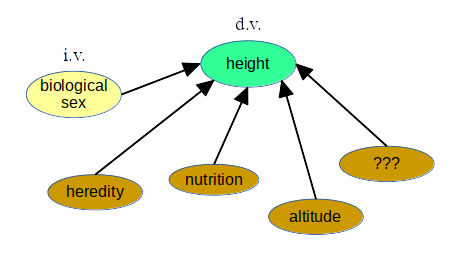
\includegraphics[width=0.7\textwidth]{sexHeight2.png}
\caption{Oh geez -- confounding variables galore? \textbf{\textit{No!}}}
\label{fig:sexHeight2}
\end{figure}

But plausible as some of those theories are, they are \textit{not} confounding
variables! These are simply \textit{other factors that may affect the d.v.}
Sure, they may also play a causal role in determining a person's height, but
they do \textit{not} invalidate our finding about sex and height.

For them to truly be confounders, they would have to affect the yellow
\textit{and} the green variable, and I'm pretty sure they do not. Do tall
parents tend to bear more sons, and short parents more daughters? If not, this
isn't a confounder. Do boys have more nutritious diets than girls? (In some
parts of the world, that may unfortunately be true, but I don't believe it is
in our country.) So that one isn't a confounder either. Having additional
causes of an effect does not nullify a genuine effect. Only a lurking variable
that pulls the marionette strings of both i.v.~and d.v.~can do that.

\section{Dealing with confounding factors}

\index{confounding factor}
\index{variable!confounding}

\label{smart}
Confounding factors are evil, and we must deal with them seriously. There are
essentially two ways to do that: one that requires us to be smart, and one that
requires us to have money.

\subsection{Controlling for a confounding factor}

\index{control (for a variable)}
\index{stratification}

If we anticipate that a certain variable may be a confounding factor, we can
\textbf{control} for it. There are several techniques for this, some of which
you'll learn in your statistics class, but the simplest one to understand
involves \textbf{stratification}.

\index{pinterest}

Let's make a silly example this time. We'll go back to the earlier pinterest
theme. I think I've noticed over the past few years that the heavy pinterest
users I know seem to almost always have long hair. I've developed a hypothesis
about this, which involves theories about how protein filaments in follicles
with longer protrusions lead to certain chemical changes in the brain. These
mind alterations, if unchecked, lead to increased creativity, craftiness, and a
desire to share artistic creations with other like-minded individuals. Further,
these aesthetic desires manifest themselves in increased usage of the
\texttt{pinterest.com} website, as measured in number of logins per day.

My theory is thus reflected in the causal diagram in
Figure~\ref{fig:hairPinterest}. Study it carefully.

\begin{figure}[ht]
\centering
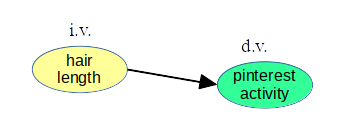
\includegraphics[width=0.6\textwidth]{hairPinterest.png}
\caption{A theory about how hair length impacts the number of times a person
logs on to pinterest each day.}
\label{fig:hairPinterest}
\end{figure}

\medskip
Now of course this follicle stuff is bogus. I'm using an extreme example to
make a point. Quick, can you come up with a possible confounding factor? Yeah,
drr: \textit{gender}. It's undoubtedly true that women tend to (but don't
always) have longer hair than men, and it's undoubtedly true that
\texttt{pinterest.com} is a website that tends to appeal to (but not
exclusively to) women. And causality-wise, the arrows obviously flow from
gender, not to it: the pinterest login screen doesn't change your gender, and a
man won't turn into a woman simply by growing his hair long (although a
transgender woman might grow her hair long as a signal of her underlying gender
change.) 

Put that all together, and you get the much more plausible causal diagram in
Figure~\ref{fig:hairPinterest2}.

\begin{figure}[ht]
\centering
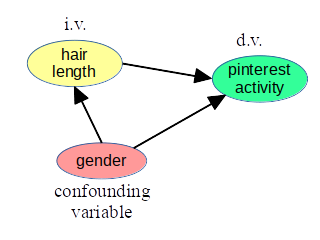
\includegraphics[width=0.6\textwidth]{hairPinterest2.png}
\caption{An alternative theory that holds that a person's gender influences
both their long-haired-ness and their pinterest-ness.}
\label{fig:hairPinterest2}
\end{figure}


\index{control (for a variable)}
\index{stratification}

Now then. Controlling for a confounding variable through stratification is done
by considering the objects of the study in \textit{groups}, comparing
\textit{only those who have the same (or similar) value for the confounding
variable.}

In this case, we would separate the men from the women in our study. Looking at
\textit{just the men}, we would ask, ``is longer hair associated with frequency
of pinterest logins?'' Then we would do the same, looking at \textit{just the
women.} Only if Python reported that both of these separate groups illustrated
such a trend would we (tentatively) conclude, ``hair length itself does play a
role in causing pinterest activity, \textit{even when controlling for
gender.}''

Do the thought experiment to see if you agree. I know the whole follicle theory
struck you as dumb (and hopefully, a little funny) to begin with. ``Of
\textit{course},'' you said to yourself, ``it's gender, not hair length, that's
drawing users to pinterest, dummy!'' But suppose we \textit{did} perform that
stratification technique, and discovered that the association actually
\textit{did} hold in both cases. Would that give it more credence in your mind?
It ought to. By stratifying, we've eliminated gender from the picture entirely,
and now we're faced with the facts that those with longer hair -- regardless of
gender -- log on to pinterest more often. 

\index{association}

Now I wrote the word ``tentatively'' a couple paragraphs ago, because there are
still some caveats. For one, we don't actually know that the causality goes in
the stated direction. Removing the gender confounder, we confirmed that there
is still an association between hair length and pinterest, but that association
might translate into a $B \rightarrow A$ phenomenon. Perhaps users who log on
to pinterest a lot see a lot of long-haired users, and (consciously or not)
decide to grow their own hair out as a result? That actually sounds more
plausible than the original silly theory. Either way, we can't confirm the
direction just by stratifying.

The other caveat is even more important, because it's more pervasive: just
because we got rid of one confounding variable doesn't mean there aren't
others. The whole ``control for a variable'' approach requires us \textit{to
anticipate in advance} what the possible confounding factors would be. This is
why I said back on p.~\pageref{smart} that this approach requires the
experimenter to be smart.

\subsection{Running a controlled experiment}

\index{controlled experiment}
\index{observational study}

The other way to deal with confounding variables is to run a \textbf{controlled
experiment} instead of an \textbf{observational study}. I jokingly said on
p.~\pageref{smart} that this option requires the experimenter to have money.
Let me explain.

\index{data-generating process (DGP)}
An observational study is one in which data is produced by naturally occurring
processes (we'll call them \textbf{data-generating processes}, or
\textbf{DGPs}) and then collected by the researcher.
Crucially, the experimenter plays no role in influencing what any of the
variable values are, whether that be the i.v.~, the d.v.~, other related
variables, or even possible confounders. Everything just is what it is, and the
researcher is simply observing.

Now at first this sounds like the best of all possible worlds. Scientists are
supposed to be objective, and to do everything they can to avoid biasing the
results, right? True, but the sad fact is that \textit{every observational
study has potential confounding factors} and there's simply no foolproof way to
account for them all. If you \textit{knew} them all, you could potentially
account for them. But in general we don't know. It all hinges on our
cleverness, which is a bit like rolling the dice.

\index{randomization!of experimental subjects}
\index{controlled experiment}

A controlled experiment, on the other hand, is one in which \textit{the
researcher decides what the value of the i.v.~will be for each object of
study.} She normally does this randomly, which is why this technique is called
\textbf{randomization}.

Now controlled experiments bear some good news and some bad news. First, the
good news, which is incredibly good, actually: \textit{a controlled experiment
automatically eliminates \underline{every} possible confounding factor, whether
you thought of it or not.} Wow: magic! We get this boon because of how the
i.v.~works. The researcher's coin flip is the \textit{sole} determinant of who
gets which i.v.~value. That means that no other factor can be ``upstream'' of
the coin flip and influence it in any way. And this in turn nullifies all
possible confounding factors, since as you recall, a confounder must affect
both the i.v.~and the d.v.

The catch is that controlled experiments can be very expensive to run, and in
many cases can't be run at \textit{all}. Consider the barbecue example from
p.~\pageref{barbecue}. To carry out a controlled experiment, we would have to:

\begin{compactenum}
\item Recruit participants to our study, and get their informed consent.
\item Pay them some \$\$ for their trouble.
\item For each participant, flip a coin. If it comes up heads, \textit{that
person must eat barbecue three times per week for the next ten years.} If it's
tails, \textit{that person must never eat barbecue for the next ten years.}
\item At the end of the ten years, measure how many barbecuers and
non-barbecuers have cancer.
\end{compactenum}

There's a question of this even being ethical: if we suspect that eating
barbecue can cause cancer, is it okay to ``force'' participants to eat it? Even
past that point, however, there's the expense. Ask yourself: if you were a
potential participant in this experiment, how much money would you demand in
step 2 to change your lifestyle to this degree? You might love barbecue, or you
might hate it, but either way, it's a coin flip that makes your decision for
you. That's a costly and intrusive change to make.

Other scenarios are even worse, because they're downright impossible. We can't
flip coins and make (at random) half of our experimental subjects male
and the other half female. We can't (or at least, shouldn't) randomly decide
our participants' political affiliations, making one random half be Democrats
and the others Republicans. And we certainly can't dictate to the nations of
the world to emit large quantities of greenhouse gases in some years and small
quantities in others, depending on our coin flip for that year.

Bottom line: if you can afford to gather data from a controlled experiment
rather than an observational study, always choose to do so. Unfortunately, it
won't always be possible, and we'll have to rest on the uneasy assumption that
we successfully predicted in advance all the important confounding variables
and controlled for them.

\section{Spurious associations}

\index{spurious association}
\index{association!spurious}

Okay, back to Figure~\ref{fig:causalityTypes} on
p.~\pageref{fig:causalityTypes}. The other item I'd like to point out in that
table is the last one, which is called a \textbf{spurious association}. This is
written as ``$A \not\rightarrow B$,'' with the arrow crossed out. And it simply
means ``nope, none of the above: these variables actually aren't associated at
all.''

You might be scratching your head at that one. Didn't I tell you
(p.~\pageref{pythonAssociation}) that Python is smart enough to tell us
definitively whether or not two variables are associated? That was supposed to
be the easy part; the hard part was only in figuring out what \textit{causes}
that association. But now I'm saying that associations might not be
associations, and Python is powerless to know the difference!

\index{IQ}
The root cause of this state of affairs is obvious once you see it, and it has
to do with the ``how much more?'' questions from p.~\pageref{howMuchMore}.
Clearly, when we collect data, there's a ``luck of the draw'' component
ever-present. I might have data that suggests Republican voters have higher
income than Democratic voters...but it's of course possible that I just
happened to poll some richer Republicans and some poorer Democrats. Suppose I
told you I thought women were on average smarter than men, and in my random
sample the average men's IQ was 102.7 and the average woman's was 103.5. The
women's was indeed greater...but is that \textit{enough} greater? Is the
difference explainable simply by the randomness of my poll?

\index{bar}
The true answer is that we can \textit{never} know for absolute certainty,
unless we can poll the entire population. (Only if we measured the IQ of every
man and every woman on planet Earth, and took the means of both groups, could
we say which one truly had the higher mean.) But what we have to do is
essentially ``set a bar'' somewhere, and then determine whether we got over it.
We could say ``only if the average IQ difference is greater than 5 points will
we conclude that there's really a difference.''

\subsection{Setting $\alpha$}

\label{alpha}

Now the procedure for determining how high to put the ``bar'' is more
complicated and more principled than that. We don't just pick a number that
seems good to us. Instead, Python will put the bar at exactly the right height,
given the level of certainty we decide to require. Some things that influence
the placement of the bar include the sample size and how variable the data is.
The thing \textit{we} specify in the bar equation, however, is \textit{how
often we're willing to draw a false conclusion.}

\index{$\alpha$ (alpha)}
\index{alpha@alpha ($\alpha$)}

That quantity is called ``$\boldsymbol{\alpha}$'' (pronounced
``\textbf{alpha}'') and is a small number between 0 and 1. Normally we'll set
$\alpha=.05$, which means: ``Python, please tell me whether the average male
and female IQs were \textit{different enough} for me to be confident that the
difference was truly a male-vs-female thing, not just an idiosyncrasy of the
people I chose for my poll. And by the way, \textit{I'm willing to be wrong 5\%
of the time about that.}''

It seems weird at first -- why would we accept drawing a faulty conclusion 5\%
of the time? Why not 0\%? But you see, we have to put the bar somewhere. If we
said, ``I never want to think there's an association when there's not one,''
Python would respond, ``well fine, if you're so worried about it then I'll
never tell you there is one.'' There has to be some kind of criterion for
judging whether a difference is ``enough,'' and $\alpha=.05$, which is ``being
suckered only 1 in 20 times'' is the most common value for social sciences.
($\alpha=.01$ is commonly used in the physical sciences.)

So, the last entry in the Figure~\ref{fig:causalityTypes} table means ``even
though the $A$ and $B$ variables aren't \textit{really} associated at all -- if
we gathered some more $A$s and some more $B$s, we'd probably detect \textit{no}
association -- you were fooled into thinking there was one because our random
sample was a bit weird.'' There's really no way around this other than being
aware it can happen, and possibly repeating our study with a different data
set to be sure of our conclusions.
